% -------------- GEOM --------------

\newcommand{\sqr}{
  \hspace{-1.5mm}
  \begin{tikzpicture}[baseline=0.2ex,scale=0.4]
    \filldraw[fill=white!25, draw=black] (0,0) rectangle (1,1);
    %\draw c d1 d2 d3 d4 d5;
  \end{tikzpicture}}


% --------------- PLAIN ----------------

\newcommand{\dts}{
  \hspace{-1.5mm}
  \begin{tikzpicture}[baseline=-0.3ex, scale=0.25]
    \tikzstyle{vertex}=[circle,fill=black, minimum size=2pt,inner sep=1pt]
    \filldraw[fill=white!25, draw=white] (-0.5,-0.5) rectangle (1,1);
    \node (d1) at (-0.2,-0.2){\texttt{.}};
    \node (d2) at (0,0.0){\texttt{.}};
    \node (d3) at (0.2,0.2){\texttt{.}};
    \node (d4) at (0.4,0.4){\texttt{.}};
    \node (d5) at (0.6,0.6){\texttt{.}};
    %\draw c d1 d2 d3 d4 d5;
  \end{tikzpicture}}

\newcommand{\bigdts}{
  \hspace{-1.5mm}
  \begin{tikzpicture}%[baseline=-0.3ex]
    \tikzstyle{vertex}=[circle,fill=black, minimum size=2pt,inner sep=1pt]
    \filldraw[fill=white!25, draw=white] (0,0) rectangle (1,1);
    \draw (0.2,0.2) -- (0.8,0.8);
  \end{tikzpicture}}


\newcommand{\xo}{
%  \hspace{-1.5mm}
  \begin{tikzpicture}[baseline=-0.3ex,scale=0.25]
    \tikzstyle{vertex}=[circle,fill=black, minimum size=2pt,inner sep=1pt]
    \filldraw[fill=white!25, draw=white] (-0.5,-0.5) rectangle (1,1);
    \node[vertex] (d) at (0.2,0.1){};
  \end{tikzpicture}}


\newcommand{\bigxo}{
%  \hspace{-1.5mm}
  \begin{tikzpicture}
    \tikzstyle{vertex}=[circle,fill=black, minimum size=2pt,inner sep=1pt]
    \filldraw[fill=white!25, draw=white] (-0.5,-0.5) rectangle (1,1);
    \filldraw[black](0.25,0.5) circle (1pt);
  \end{tikzpicture}}


\newcommand{\xdts}{
  \hspace{-1.5mm}
  \begin{tikzpicture}[baseline=-0.3ex,scale=0.25]
    \tikzstyle{vertex}=[circle,fill=black, minimum size=2pt,inner sep=1pt]
    \filldraw[fill=white!25, draw=white] (-0.5,-0.5) rectangle (1,1);
    \node (d1) at (-0.3,-0.3){\footnotesize{\texttt{+}}};
    \node (d2) at (0,0.0){\texttt{.}};
    \node (d3) at (0.2,0.2){\texttt{.}};
    \node (d4) at (0.4,0.4){\texttt{.}};
    \node (d5) at (0.6,0.6){\texttt{.}};
    %\draw c d1 d2 d3 d4 d5;
  \end{tikzpicture}}

\newcommand{\bigxdts}{
  \hspace{-1.5mm}
  \begin{tikzpicture}
    \tikzstyle{vertex}=[circle,fill=black, minimum size=2pt,inner sep=1pt]
    \filldraw[fill=white!25, draw=white] (-0.5,-0.5) rectangle (1,1);
    \filldraw[black](0.2,0.2) node{\texttt{+}};
    \draw (0.3,0.3)--(0.8,0.8);
  \end{tikzpicture}}

\newcommand{\xdtso}{
  \hspace{-1.5mm}
  \begin{tikzpicture}[baseline=-0.3ex,scale=0.25]
    \tikzstyle{vertex}=[circle,fill=black, minimum size=2pt,inner sep=1pt]
    \filldraw[fill=white!25, draw=white] (-0.5,-0.5) rectangle (1,1);
    \node (d1) at (-0.3,-0.3){\footnotesize{\texttt{+}}};
    \node (d2) at (0,0.0){\texttt{.}};
    \node (d3) at (0.2,0.2){\texttt{.}};
    \node (d4) at (0.4,0.4){\texttt{.}};
    \node (d5) at (0.7,0.7){\footnotesize{\texttt{o}}};
    %\draw c d1 d2 d3 d4 d5;
  \end{tikzpicture}}

\newcommand{\bigxdtso}{
  \hspace{-1.5mm}
  \begin{tikzpicture}%[baseline=-0.3ex]
    \tikzstyle{vertex}=[circle,fill=black, minimum size=2pt,inner sep=1pt]
    \filldraw[fill=white!25, draw=white] (-0.5,-0.5) rectangle (1,1);
    \filldraw[black](0.2,0.2) node{\texttt{+}};
    \draw (0.3,0.3)--(0.7,0.7);
    \filldraw[black](0.8,0.8) node{\texttt{o}};
  \end{tikzpicture}}

\newcommand{\dtso}{
  \hspace{-1.5mm}
  \begin{tikzpicture}[baseline=-0.3ex,scale=0.25]
    \tikzstyle{vertex}=[circle,fill=black, minimum size=2pt,inner sep=1pt]
    \filldraw[fill=white!25, draw=white] (-0.5,-0.5) rectangle (1,1);
    \node (d1) at (-0.3,-0.3){\texttt{.}};
    \node (d2) at (0,0.0){\texttt{.}};
    \node (d3) at (0.2,0.2){\texttt{.}};
    \node (d4) at (0.4,0.4){\texttt{.}};
    \node (d5) at (0.7,0.7){\footnotesize{\texttt{o}}};
    %\draw c d1 d2 d3 d4 d5;
  \end{tikzpicture}}

\newcommand{\bigdtso}{
  \hspace{-1.5mm}
  \begin{tikzpicture}%[baseline=-0.3ex]
    \tikzstyle{vertex}=[circle,fill=black, minimum size=2pt,inner sep=1pt]
    \filldraw[fill=white!25, draw=white] (-0.5,-0.5) rectangle (1,1);
    \draw (0.2,0.2)--(0.7,0.7);
    \filldraw[black](0.8,0.8) node{\texttt{o}};
  \end{tikzpicture}}

% ------------ RED ---------------------

\newcommand{\dtsred}{
  \hspace{-1.5mm}
  
\begin{tikzpicture}[baseline=-0.3ex,scale=0.25]
    \tikzstyle{vertex}=[circle,fill=black, minimum size=2pt,inner sep=1pt]
    \filldraw[fill=red!25, draw=white] (-0.5,-0.5) rectangle (1,1);
    \node (d1) at (-0.2,-0.2){\texttt{.}};
    \node (d2) at (0,0.0){\texttt{.}};
    \node (d3) at (0.2,0.2){\texttt{.}};
    \node (d4) at (0.4,0.4){\texttt{.}};
    \node (d5) at (0.6,0.6){\texttt{.}};
  \end{tikzpicture}}


\newcommand{\xored}{
 % \hspace{-1.5mm}
  
\begin{tikzpicture}[baseline=-0.3ex,scale=0.25]
    \tikzstyle{vertex}=[circle,fill=black, minimum size=2pt,inner sep=1pt]
    \filldraw[fill=red!25, draw=white] (-0.5,-0.5) rectangle (1,1);
    \node[vertex] (d) at (0.2,0.1){};
  \end{tikzpicture}}


\newcommand{\xdtsred}{
  \hspace{-1.5mm}
  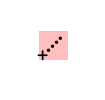
\begin{tikzpicture}[baseline=-0.3ex,scale=0.25]
    \tikzstyle{vertex}=[circle,fill=black, minimum size=2pt,inner sep=1pt]
    \filldraw[fill=red!25, draw=white] (-0.5,-0.5) rectangle (1,1);
    \node (d1) at (-0.3,-0.3){\footnotesize{\texttt{+}}};
    \node (d2) at (0,0.0){\texttt{.}};
    \node (d3) at (0.2,0.2){\texttt{.}};
    \node (d4) at (0.4,0.4){\texttt{.}};
    \node (d5) at (0.6,0.6){\texttt{.}};
    %\draw c d1 d2 d3 d4 d5;
  \end{tikzpicture}}


\newcommand{\xdtsored}{
  \hspace{-1.5mm}
  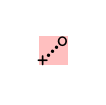
\begin{tikzpicture}[baseline=-0.3ex,scale=0.25]
    \tikzstyle{vertex}=[circle,fill=black, minimum size=2pt,inner sep=1pt]
    \filldraw[fill=red!25, draw=white] (-0.5,-0.5) rectangle (1,1);
    \node (d1) at (-0.3,-0.3){\footnotesize{\texttt{+}}};
    \node (d2) at (0,0.0){\texttt{.}};
    \node (d3) at (0.2,0.2){\texttt{.}};
    \node (d4) at (0.4,0.4){\texttt{.}};
    \node (d5) at (0.7,0.7){\footnotesize{\texttt{o}}};
    %\draw c d1 d2 d3 d4 d5;
  \end{tikzpicture}}

\newcommand{\dtsored}{
  \hspace{-1.5mm}
  
\begin{tikzpicture}[baseline=-0.3ex,scale=0.25]
    \tikzstyle{vertex}=[circle,fill=black, minimum size=2pt,inner sep=1pt]
    \filldraw[fill=red!25, draw=white] (-0.5,-0.5) rectangle (1,1);
    \node (d1) at (-0.3,-0.3){\texttt{.}};
    \node (d2) at (0,0.0){\texttt{.}};
    \node (d3) at (0.2,0.2){\texttt{.}};
    \node (d4) at (0.4,0.4){\texttt{.}};
    \node (d5) at (0.7,0.7){\footnotesize{\texttt{o}}};
    %\draw c d1 d2 d3 d4 d5;
  \end{tikzpicture}}

% ------------ GREEN ---------------------

\newcommand{\dtsgreen}{
  \hspace{-1.5mm}
  
\begin{tikzpicture}[baseline=-0.3ex,scale=0.25]
    \tikzstyle{vertex}=[circle,fill=black, minimum size=2pt,inner sep=1pt]
    \filldraw[fill=green!25, draw=white] (-0.5,-0.5) rectangle (1,1);
    \node (d1) at (-0.2,-0.2){\texttt{.}};
    \node (d2) at (0,0.0){\texttt{.}};
    \node (d3) at (0.2,0.2){\texttt{.}};
    \node (d4) at (0.4,0.4){\texttt{.}};
    \node (d5) at (0.6,0.6){\texttt{.}};
  \end{tikzpicture}}


\newcommand{\xogreen}{
 % \hspace{-1.5mm}
  
\begin{tikzpicture}[baseline=-0.3ex,scale=0.25]
    \tikzstyle{vertex}=[circle,fill=black, minimum size=2pt,inner sep=1pt]
    \filldraw[fill=green!25, draw=white] (-0.5,-0.5) rectangle (1,1);
    \node[vertex] (d) at (0.2,0.1){};
  \end{tikzpicture}}


\newcommand{\xdtsgreen}{
  \hspace{-1.5mm}
  
\begin{tikzpicture}[baseline=-0.3ex,scale=0.25]
    \tikzstyle{vertex}=[circle,fill=black, minimum size=2pt,inner sep=1pt]
    \filldraw[fill=green!25, draw=white] (-0.5,-0.5) rectangle (1,1);
    \node (d1) at (-0.3,-0.3){\footnotesize{\texttt{+}}};
    \node (d2) at (0,0.0){\texttt{.}};
    \node (d3) at (0.2,0.2){\texttt{.}};
    \node (d4) at (0.4,0.4){\texttt{.}};
    \node (d5) at (0.6,0.6){\texttt{.}};
    %\draw c d1 d2 d3 d4 d5;
  \end{tikzpicture}}


\newcommand{\xdtsogreen}{
  \hspace{-1.5mm}
  
\begin{tikzpicture}[baseline=-0.3ex,scale=0.25]
    \tikzstyle{vertex}=[circle,fill=black, minimum size=2pt,inner sep=1pt]
    \filldraw[fill=green!25, draw=white] (-0.5,-0.5) rectangle (1,1);
    \node (d1) at (-0.3,-0.3){\footnotesize{\texttt{+}}};
    \node (d2) at (0,0.0){\texttt{.}};
    \node (d3) at (0.2,0.2){\texttt{.}};
    \node (d4) at (0.4,0.4){\texttt{.}};
    \node (d5) at (0.7,0.7){\footnotesize{\texttt{o}}};
    %\draw c d1 d2 d3 d4 d5;
  \end{tikzpicture}}

\newcommand{\dtsogreen}{
  \hspace{-1.5mm}
  
\begin{tikzpicture}[baseline=-0.3ex,scale=0.25]
    \tikzstyle{vertex}=[circle,fill=black, minimum size=2pt,inner sep=1pt]
    \filldraw[fill=green!25, draw=white] (-0.5,-0.5) rectangle (1,1);
    \node (d1) at (-0.3,-0.3){\texttt{.}};
    \node (d2) at (0,0.0){\texttt{.}};
    \node (d3) at (0.2,0.2){\texttt{.}};
    \node (d4) at (0.4,0.4){\texttt{.}};
    \node (d5) at (0.7,0.7){\footnotesize{\texttt{o}}};
    %\draw c d1 d2 d3 d4 d5;
  \end{tikzpicture}}
